% ------------------------------------------------------------------------------
% TYPO3 Version 10.1 - What's New (Italian Version)
%
% @license	Creative Commons BY-NC-SA 3.0
% @link		http://typo3.org/download/release-notes/whats-new/
% @language	Italian
% ------------------------------------------------------------------------------

\section{Interfaccia utente di Backend}
\begin{frame}[fragile]
	\frametitle{Interfaccia utente di Backend}

	\begin{center}\huge{Capitolo 1:}\end{center}
	\begin{center}\huge{\color{typo3darkgrey}\textbf{Interfaccia utente di Backend}}\end{center}

\end{frame}

% ------------------------------------------------------------------------------
% Feature | 89115 | Auto slug update and redirect creation on slug change

\begin{frame}[fragile]
	\frametitle{Interfaccia utente di Backend}
	\framesubtitle{Aggiornamenti e redirect degli slug (1)}

	\begin{itemize}
		\item Quando un utente di backend cambia il path URL di una pagina (il cosidetto "slug"),
			il vecchio URL non è più raggiungibile.
		\item Questo comporta un errore "pagina non trovata" per questa pagina,
			compresi gli url di tutte le sottopagine.
	\end{itemize}

	\begin{figure}
		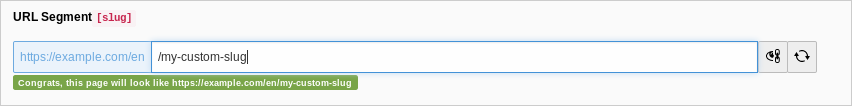
\includegraphics[width=0.80\linewidth]{BackendUserInterface/89115b-AutoSlugUpdateAndRedirectCreationOnSlugChange.png}
	\end{figure}

	\begin{itemize}
		\item Da TYPO3 v10.1, due azioni impediscono che ciò accada

			\begin{itemize}
				\item Gli slug per tutte le sottopagine sono aggiornate automaticamente
				\item E' creato un redirect dal vecchio url al nuovo url
			\end{itemize}

	\end{itemize}

\end{frame}

% ------------------------------------------------------------------------------
% Feature | 89115 | Auto slug update and redirect creation on slug change

\begin{frame}[fragile]
	\frametitle{Interfaccia utente di Backend}
	\framesubtitle{Aggiornamenti e redirect degli slug (2)}

	\begin{itemize}
		\item Gli utenti di backend sono informati di queste azioni e possono
			ripristinare facilmente le modifiche con un clic, se necessario:

	\end{itemize}

	\begin{figure}
		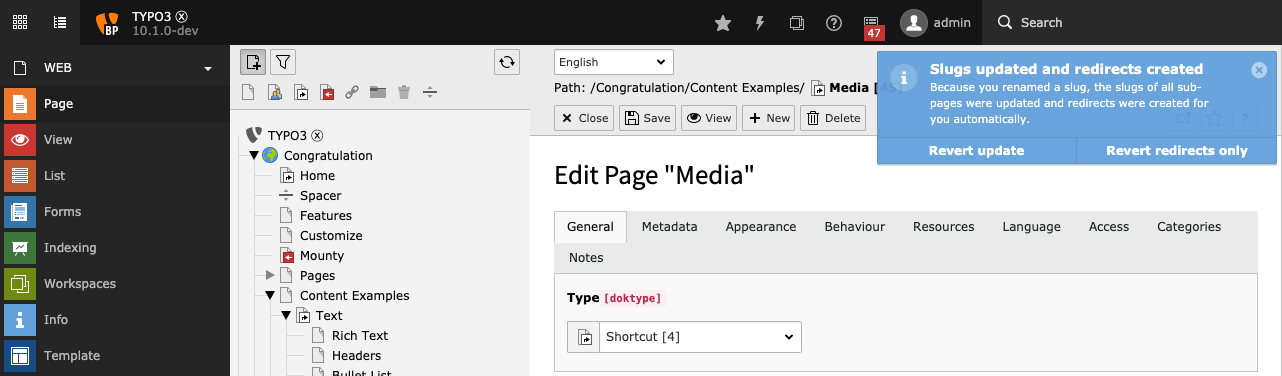
\includegraphics[width=0.80\linewidth]{BackendUserInterface/89115c-AutoSlugUpdateAndRedirectCreationOnSlugChange.png}
	\end{figure}

\end{frame}

% ------------------------------------------------------------------------------
% Feature | 85918 | Hide in menu / Show in menu entry for pages in context menu

\begin{frame}[fragile]
	\frametitle{Interfaccia utente di Backend}
	\framesubtitle{Nascondi/Visualizza in Menu}

	E' stata aggiunta una nuova voce al menu di scelta rapida per nascondere/visualizzare le pagine nel menu.

	\begin{figure}
		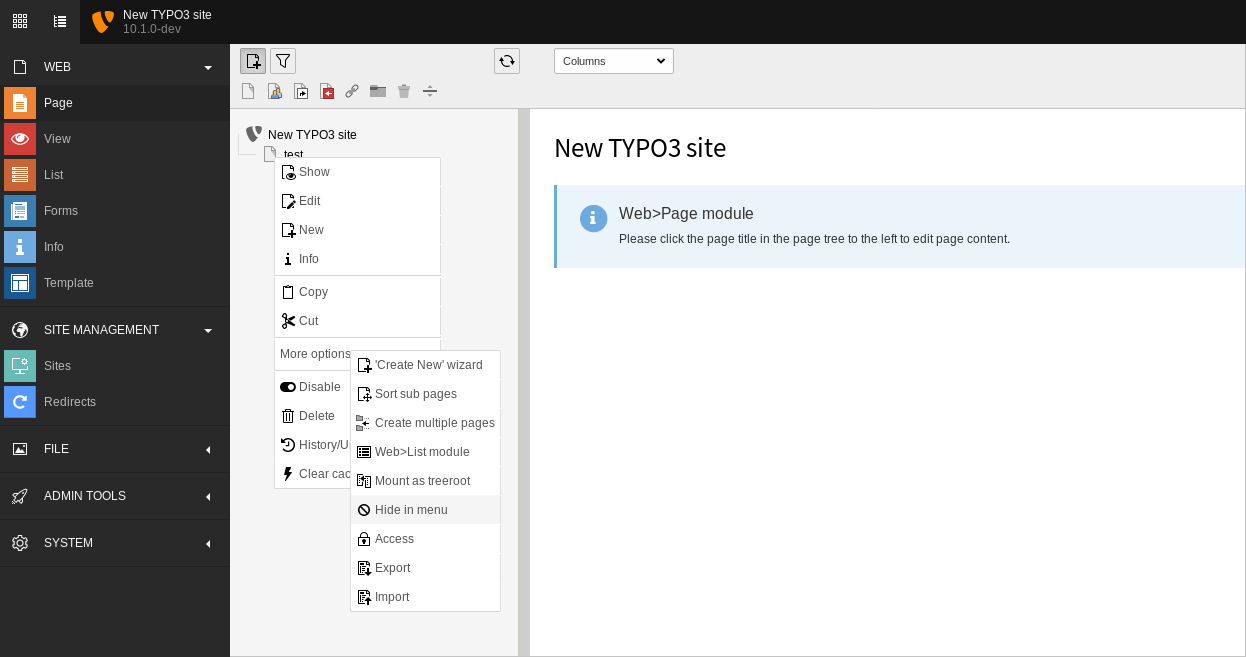
\includegraphics[width=0.80\linewidth]{BackendUserInterface/85918-HideShowInMenu-InContextMenu.png}
	\end{figure}

\end{frame}

% ------------------------------------------------------------------------------
